\chapter{Einleitung}
Im Fach Fortgeschrittene Internetanwendungen haben wir uns im Rahmen einer studentischen Projektarbeit mit dem Thema Navigation und Lokalisierung innerhalb von Geb�uden besch�ftigt. Dabei beschr�nkte sich das Ziel unseres Projekts auf die Navigation im Geb�ude der Westf�lischen Hochschule am Campus Bocholt.

Dazu stellten wir uns zu Projektbeginn eine Karte des Geb�udes vor, auf der alle m�glichen Navigationsziele eingezeichnet sind. Bei der Auswahl eines Navigationsziels sollte nach unseren Vorstellungen eine entsprechende Wegbeschreibung eingeblendet werden, die uns von unserem aktuellen Standpunkt zum gew�nschten Ziel f�hrt.

Um dieses Ziel zu erreichen, mussten wir uns mit verschiedenen Problemstellungen auseinandersetzen. Zun�chst einmal war es n�tig das Geb�ude vollst�ndig in unserem System zu erfassen. Zum anderen mussten wir die aktuelle Position innerhalb des Geb�udes ermitteln, um diese ebenfalls auf der Karte abbilden zu k�nnen.

\section{Motivation}
Motiviert durch die Tatsache, dass vor allem neue Studenten und Ortsunkundige sich nicht im Geb�ude der Hochschule zurecht finden, entstand die Idee eine Navigationssoftware zu entwickeln. Basierend auf folgenden Anwendungsf�llen:

\begin{figure}[H]
\centering
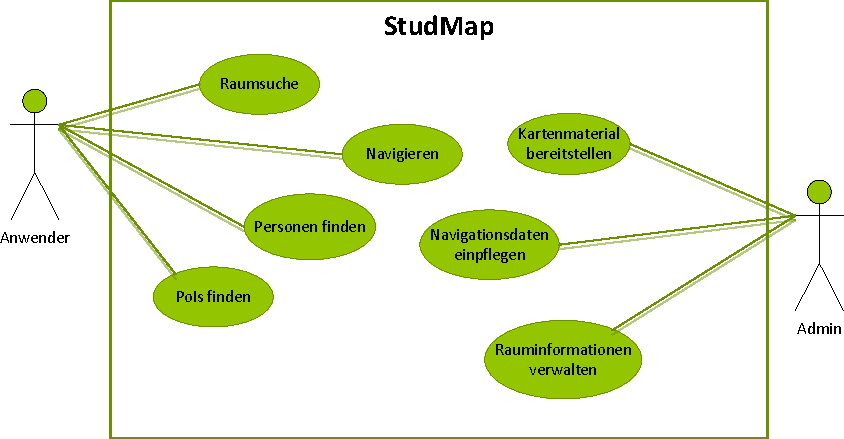
\includegraphics[width=\linewidth]{../Bilder/UseCaseDiagram}
\label{fig:UseCaseDiagram}
\end{figure}

Der Anwender hat in den meisten F�llen Interesse daran, zu besonderen
Orte, die sogenannten Points of Interest (Abk�rzung PoI), der Hochschule zu gelangen (z.B. Mensa, Dekanat). Neben diesen wird auch gelegentlich nach den verbleibenden R�umen des Geb�udes gesucht (z.B. Seminarr�ume).
F�r das Auffinden von und die Navigation zu diesen Orten wollen wir eine Anwendung entwickeln. Dar�ber hinaus sollen auf der Karte angemeldete Benutzer zu finden sein\footnote{Siehe \href{http://de.wikipedia.org/wiki/Begriffe\_der\_Harry-Potter-Romane\#Karte\_des\_Rumtreibers}{Karte des Rumtreibers}}.

Damit ein solches System funktioniert ben�tigt dies einen Administrator, der sich um das Kartenmaterial und um die Datenpflege k�mmert.

\section{Projektorganisation}
Als Plattform f�r unser Projekt verwenden wir Google Code:\\
\href{https://code.google.com/p/studmap/}{https://code.google.com/p/studmap/}

Dort nutzen wir das SVN Repository zur Quellcode Ablage und den Issue Tracker zur Verwaltung von Benutzeranforderungen und Fehlern. Wir haben uns in unserem Projekt f�r eine agile Projektorganisation nach dem Vorbild von Scrum entschieden und den Issue Tracker entsprechend konfiguriert. So stehen uns die Issue Typen User Story, Task und Bug zur Verf�gung. Zus�tzlich haben wir noch vier Kategorien eingef�hrt: ProductBacklog, SprintBacklog, OpenBugs und OpenTasks. Mittels der Kategorien k�nnen wir die verschiedenen Issues besser strukturieren.

Kurz nach Beginn des Projektes haben wir die Benutzeranforderungen in Form von User Stories\footnote{Siehe \href{https://code.google.com/p/studmap/issues/list?can=1\&q=type=UserStory\&colspec=ID\%20Type\%20Status\%20Priority\%20PartOf\%20Component\%20Owner\%20Summary}{Google Code}}
angelegt und dem ProductBacklog zugewiesen. F�r dieses Projekt haben wir uns auf Sprints mit einer Dauer von jeweils zwei Wochen geeinigt. Zu Beginn eines jeden Sprints haben wir entsprechende User Stories in den SprintBacklog �bertragen und abgearbeitet.